\section{Experiments}\label{sec::expr}

In the experiments, we emphasized there were no corresponding images in the different domains in the training sets. CoGAN learned the joint distributions without correspondence supervision. We were unaware of existing approaches with the same capability and hence did not compare CoGAN with prior works. Instead, we compared it to a conditional GAN to demonstrate its advantage. Recognizing that popular performance metrics for evaluating generative models all subject to issues~\cite{theis2015note}, we adopted a pair image generation performance metric for comparison. Many details including the network architectures and additional experiment results are given in the supplementary materials. An implementation of CoGAN is available in \url{https://github.com/mingyuliutw/cogan}. 


\begin{figure}[t]
\centering
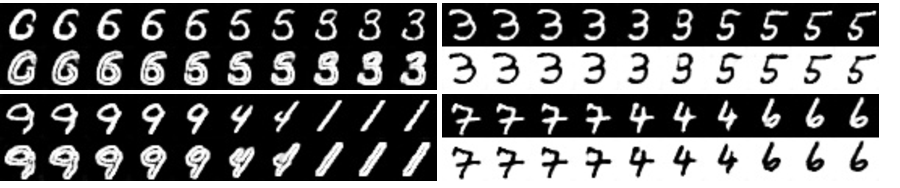
\includegraphics[trim=0.0in 0.12in 0.1in 0.in, width=1.0\textwidth]{result_mnist_small.pdf}
\caption{\small Left (Task $\mathbb{A}$): generation of digit and corresponding edge images. Right (Task $\mathbb{B}$): generation of digit and corresponding negative images. Each of the top and bottom pairs was generated using the same input noise. We visualized the results by traversing in the input space.}
\label{fig::result_mnist}
\centering
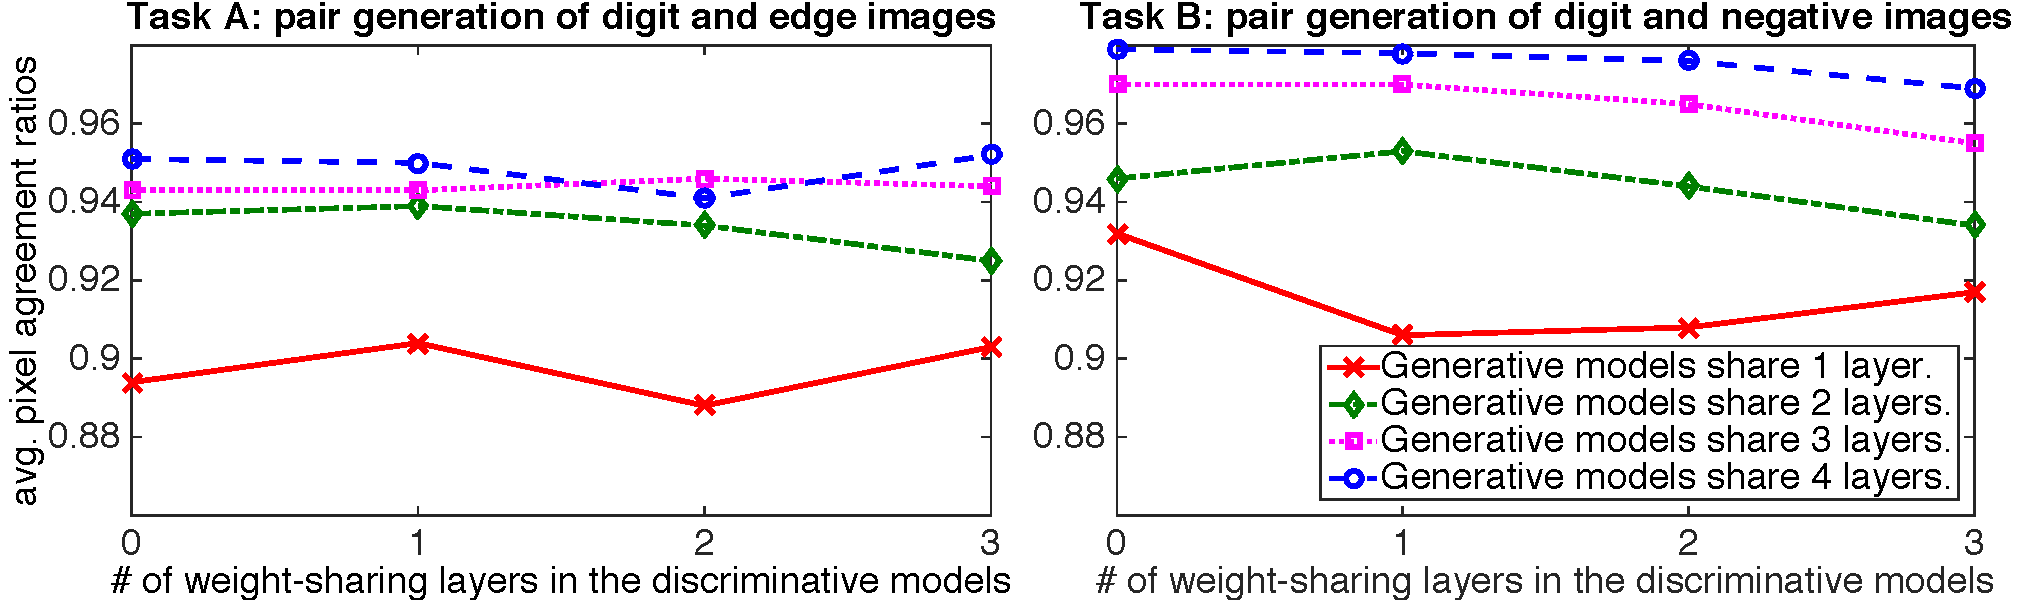
\includegraphics[trim=0.in 0.1in 0.in 0in, width=1.0\textwidth]{weight-sharing.pdf}
\caption{\small The figures plot the average pixel agreement ratios of the CoGANs with different weight-sharing configurations for Task $\mathbb{A}$ and $\mathbb{B}$. The larger the pixel agreement ratio the better the pair generation performance. We found that the performance was positively correlated with the number of weight-sharing layers in the generative models but was uncorrelated to the number of weight-sharing layers in the discriminative models. CoGAN learned the joint distribution without weight-sharing layers in the discriminative models.}
\label{fig::quantitative_digit}
\vspace{-2mm}
\end{figure}

{\bf Digits:} We used the MNIST training set to train CoGANs for the following two tasks. Task $\mathbb{A}$ is about learning a joint distribution of a digit and its edge image. Task $\mathbb{B}$ is about learning a joint distribution of a digit and its negative image. In Task $\mathbb{A}$, the 1st domain consisted of the original handwritten digit images, while the 2nd domain consisted of their edge images. We used an edge detector to compute training edge images for the 2nd domain. In the supplementary materials, we also showed an experiment for learning a joint distribution of a digit and its 90-degree in-plane rotation.

We used deep convolutional networks to realized the CoGAN. The two generative models had an identical structure; both had 5 layers and were fully convolutional. The stride lengths of the convolutional layers were fractional. The models also employed the batch normalization processing~\cite{ioffe2015batch} and the parameterized rectified linear unit processing~\cite{he2015delving}. We shared the parameters for all the layers except for the last convolutional layers. For the discriminative models, we used a variant of LeNet~\cite{lecun1998gradient}. The inputs to the discriminative models were batches containing output images from the generative models and images from the two training subsets (each pixel value is linearly scaled to $[0\medspace1]$). 

We divided the training set into two equal-size {\it non-overlapping} subsets. One was used to train $\text{GAN}_1$ and the other was used to train $\text{GAN}_2$. We used the ADAM algorithm~\cite{kingma2014adam} for training and set the learning rate to 0.0002, the 1st momentum parameter to 0.5, and the 2nd momentum parameter to 0.999 as suggested in~\cite{radford2015unsupervised}. The mini-batch size was 128. We trained the CoGAN for 25000 iterations. These hyperparameters were fixed for all the visualization experiments. 

The CoGAN learning results are shown in Figure~\ref{fig::result_mnist}. We found that although the CoGAN was trained without corresponding images, it learned to render corresponding ones for both Task $\mathbb{A}$ and $\mathbb{B}$. This was due to the weight-sharing constraint imposed to the layers that were responsible for decoding high-level semantics. Exploiting the correspondence between the two domains allowed $\text{GAN}_1$ and $\text{GAN}_2$ to utilize more capacity in the networks to better fit the training data. Without the weight-sharing constraint, the two GANs just generated two unrelated images in the two domains.

{\bf Weight Sharing:} We varied the numbers of weight-sharing layers in the generative and discriminative models to create different CoGANs for analyzing the weight-sharing effect for both tasks. Due to lack of proper validation methods, we did a grid search on the training iteration hyperparameter and reported the best performance achieved by each network. For quantifying the performance, we transformed the image generated by $\text{GAN}_1$ to the 2nd domain using the same method employed for generating the training images in the 2nd domain. We then compared the transformed image with the image generated by $\text{GAN}_2$. A perfect joint distribution learning should render two identical images. Hence, we used the ratios of agreed pixels between 10K pairs of images generated by each network (10K randomly sampled $\mathbf{z}$) as the performance metric. We trained each network 5 times with different initialization weights and reported the average pixel agreement ratios over the 5 trials for each network. The results are shown in Figure~\ref{fig::quantitative_digit}. We observed that the performance was positively correlated with the number of weight-sharing layers in the generative models. With more sharing layers in the generative models, the rendered pairs of images resembled true pairs drawn from the joint distribution more. We also noted that the performance was uncorrelated to the number of weight-sharing layers in the discriminative models. However, we still preferred discriminator weight-sharing because this reduces the total number of network parameters.

{\bf Comparison with Conditional GANs:} We compared the CoGAN with the conditional GANs~\cite{mirza2014conditional}. We designed a conditional GAN with the generative and discriminative models identical to those in the CoGAN. The only difference was the conditional GAN took an additional binary variable as input, which controlled the domain of the output image. When the binary variable was 0, it generated an image resembling images in the 1st domain; otherwise, it generated an image resembling images in the 2nd domain. Similarly, no pairs of corresponding images were given during the conditional GAN training. We applied the conditional GAN to both Task  $\mathbb{A}$ and $\mathbb{B}$ and hoped to empirically answer whether a conditional model can be used to learn to render corresponding images with correspondence supervision. The pixel agreement ratio was used as the performance metric. The experiment results showed that for Task $\mathbb{A}$, CoGAN achieved an average ratio of {\bf 0.952}, outperforming 0.909 achieved by the conditional GAN. For Task $\mathbb{B}$, CoGAN achieved a score of {\bf 0.967}, which was much better than 0.778 achieved by the conditional GAN. The conditional GAN just generated two different digits with the same random noise input but different binary variable values. These results showed that the conditional model failed to learn a joint distribution from samples drawn from the marginal distributions. We note that for the case that the supports of the two domains are different such as the color and depth image domains, the conditional model cannot even be applied. 

\begin{figure*}[thb!]
\centering
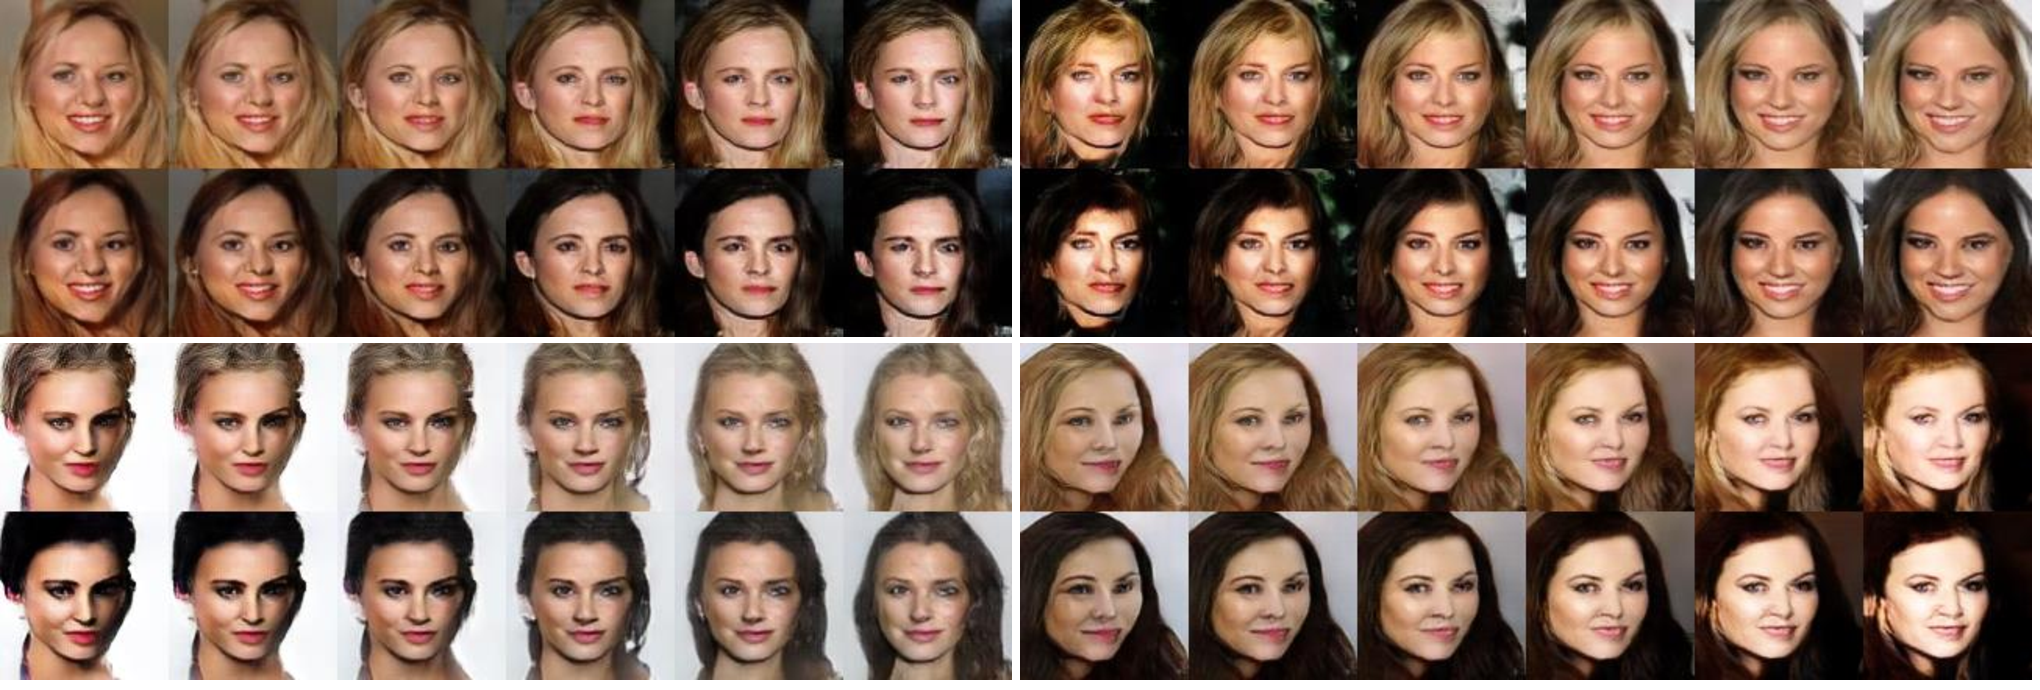
\includegraphics[trim=0in 0.0in 0in 0in, width=1.\textwidth]{result_face_blondhair_small.pdf}
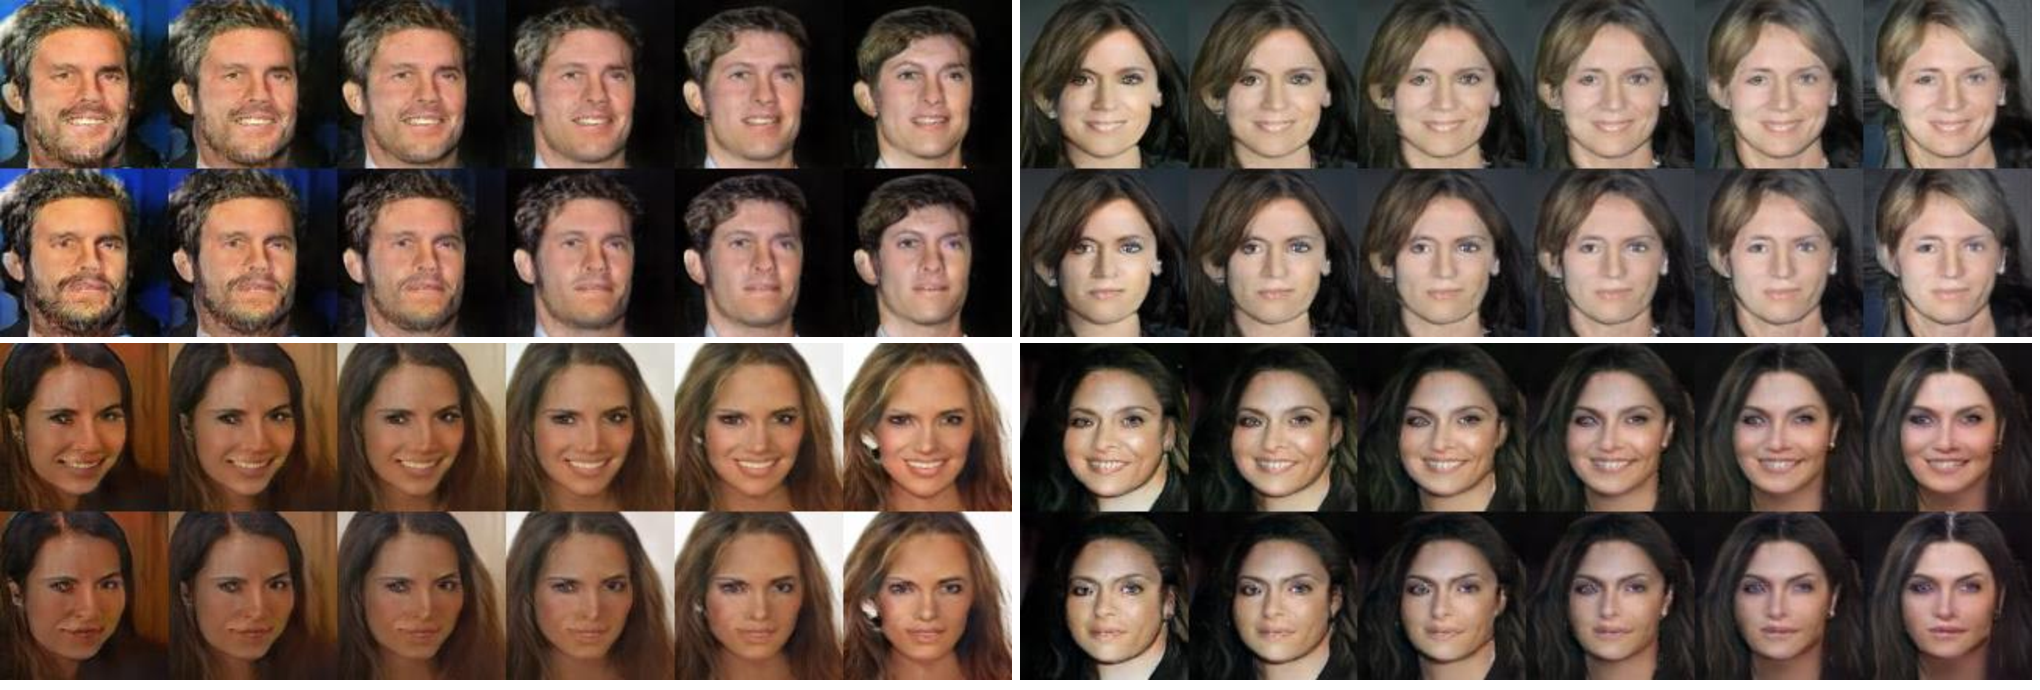
\includegraphics[trim=0in 0.0in 0in 0in, width=1.\textwidth]{result_face_smiling_small.pdf}
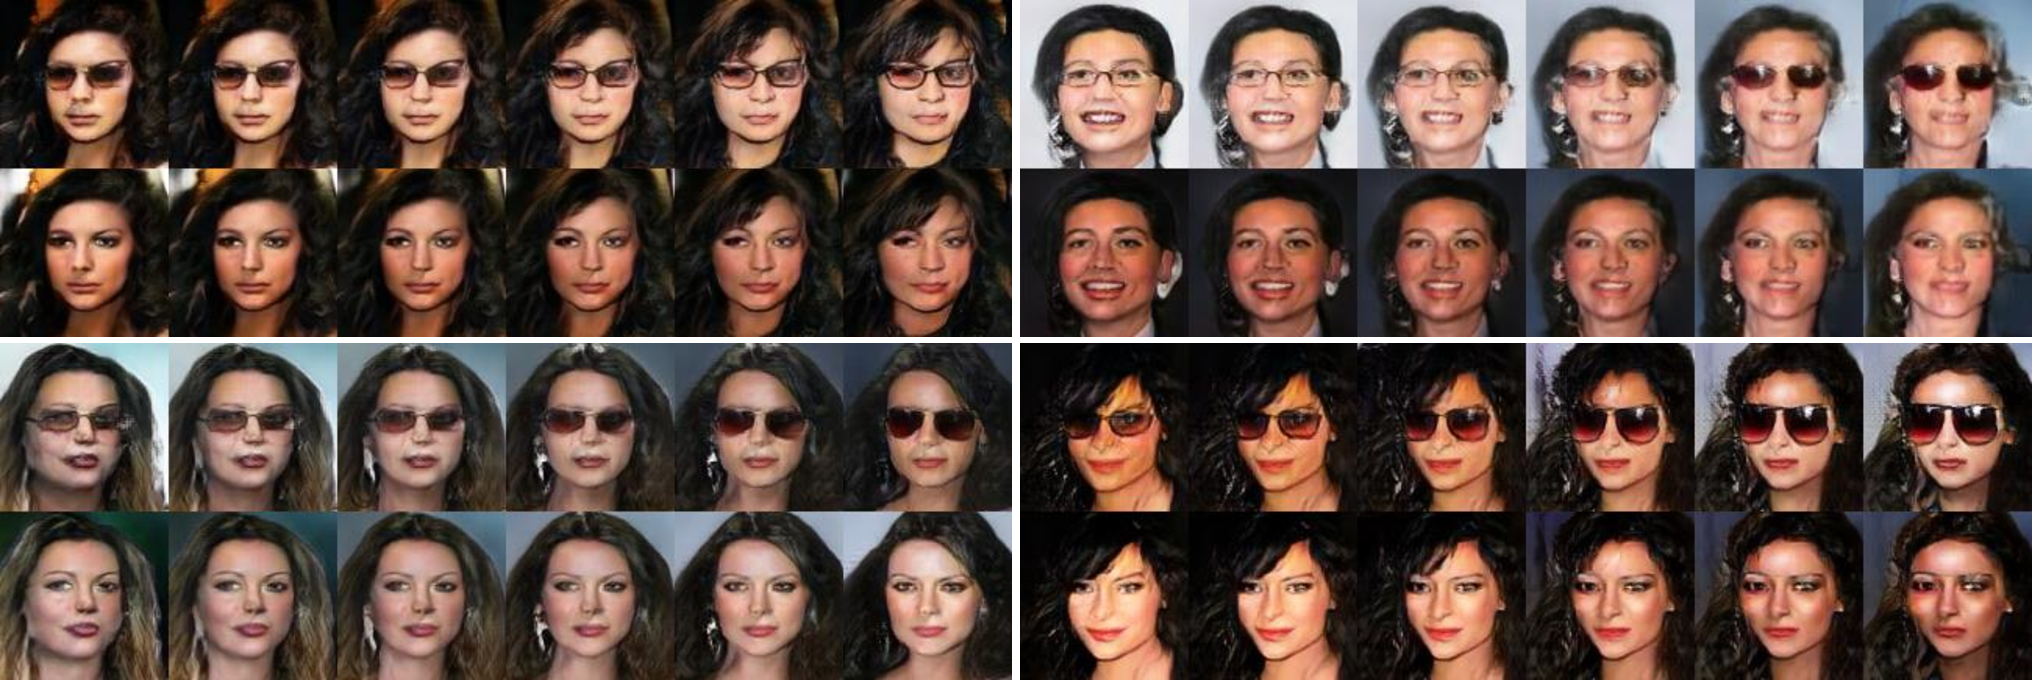
\includegraphics[trim=0in 0.2in 0in 0in, width=1.\textwidth]{result_face_eyeglasses_small.pdf}
\caption{\small Generation of face images with different attributes using CoGAN. From top to bottom, the figure shows pair face generation results for the blond-hair, smiling, and eyeglasses attributes. For each pair, the 1st row contains faces with the attribute, while the 2nd row contains corresponding faces without the attribute.}
\label{fig::result_attr_faces}
\vspace{-2mm}
\end{figure*}

{\bf Faces:} We applied CoGAN to learn a joint distribution of face images with different. We trained several CoGANs, each for generating a face with an attribute and a corresponding face without the attribute. We used the CelebFaces Attributes dataset~\cite{liu2015deep} for the experiments. The dataset covered large pose variations and background clutters. Each face image had several attributes, including blond hair, smiling, and eyeglasses. The face images with an attribute constituted the 1st domain; and those without the attribute constituted the 2nd domain. No corresponding face images between the two domains was given. We resized the images to a resolution of $132\times132$ and randomly sampled $128\times128$ regions for training. The generative and discriminative models were both 7 layer deep convolutional neural networks. 

The experiment results are shown in Figure~\ref{fig::result_attr_faces}. We randomly sampled two points in the 100-dimensional input noise space and visualized the rendered face images as traveling from one pint to the other. We found CoGAN generated pairs of corresponding faces, resembling those from the same person with and without an attribute. As traveling in the space, the faces gradually change from one person to another. Such deformations were consistent for both domains. Note that it is difficult to create a dataset with corresponding images for some attribute such as blond hair since the subjects have to color their hair. It is more ideal to have an approach that does not require corresponding images like CoGAN. We also noted that the number of faces with an attribute was often several times smaller than that without the attribute in the dataset. However, CoGAN learning was not hindered by the mismatches.

{\bf Color and Depth Images:} We used the RGBD dataset~\cite{lai2011large} and the NYU dataset~\cite{silberman2012indoor} for learning joint distribution of color and depth images. The RGBD dataset contains registered color and depth images of 300 objects captured by the Kinect sensor from different view points. We partitioned the dataset into two equal-size {\it non-overlapping} subsets. The color images in the 1st subset were used for training $\text{GAN}_1$, while the depth images in the 2nd subset were used for training $\text{GAN}_2$. There were no corresponding depth and color images in the two subsets. The images in the RGBD dataset have different resolutions. We resized them to a fixed resolution of $64\times64$. The NYU dataset contains color and depth images captured from indoor scenes using the Kinect sensor. We used the 1449 processed depth images for the depth domain. The training images for the color domain were from all the color images in the raw dataset except for those registered with the processed depth images. We resized both the depth and color images to a resolution of $176\times132$ and randomly cropped $128\times128$ patches for training. 

Figure~\ref{fig::result_rgbd} showed the generation results. We found the rendered color and depth images resembled corresponding RGB and depth image pairs despite of no registered images existed in the two domains in the training set. The CoGAN recovered the appearance--depth correspondence unsupervisedly.

\begin{figure}[t!]
\centering
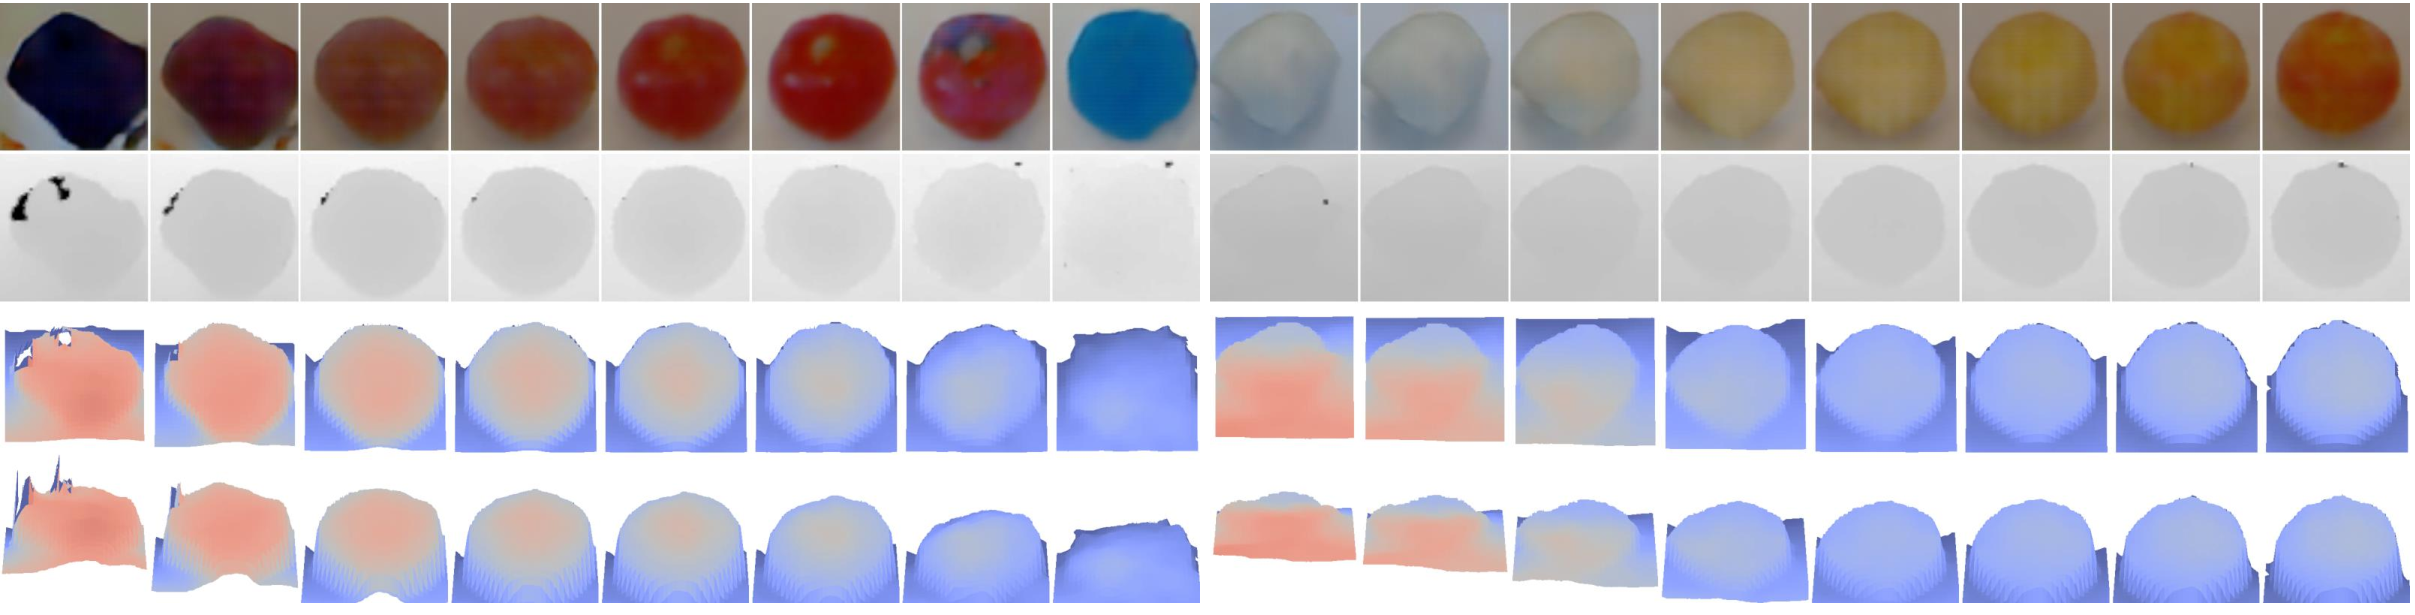
\includegraphics[trim=0in 0.1in 0in 0in, width=1.\textwidth]{result_rgbd_small.pdf}
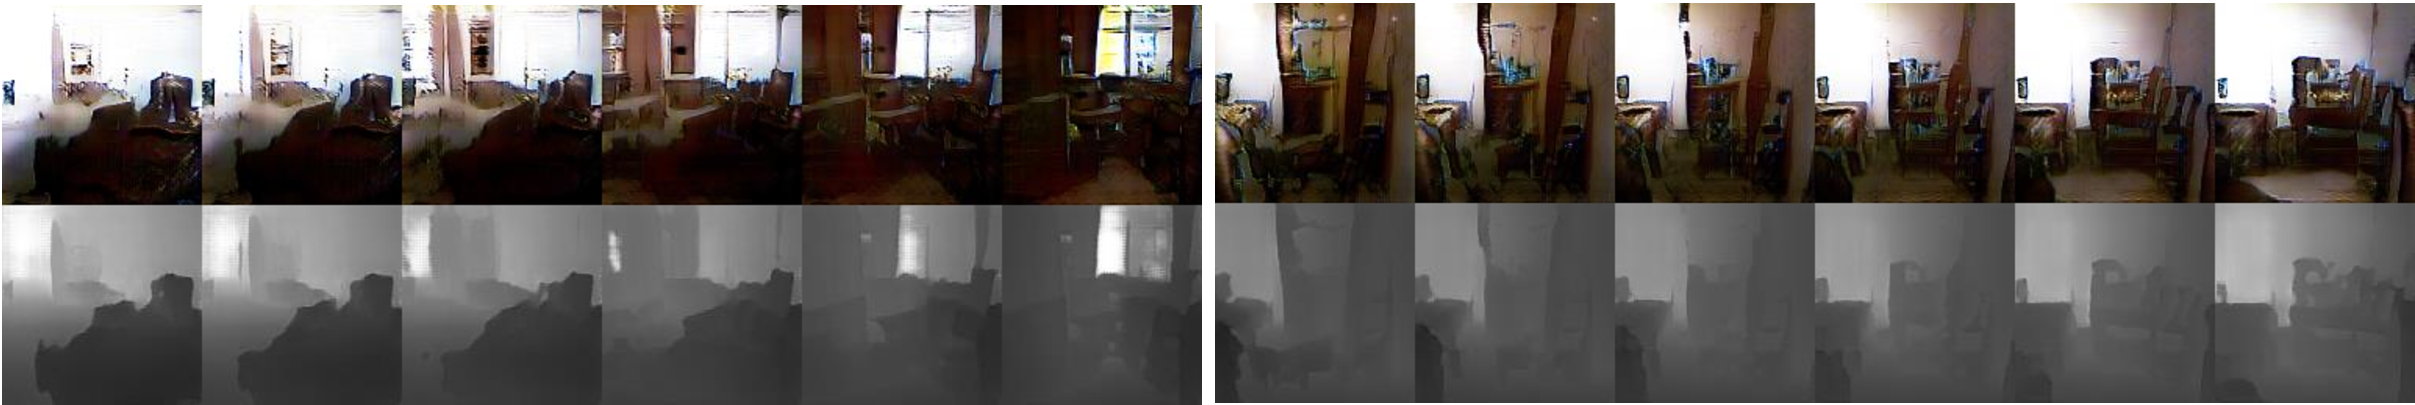
\includegraphics[trim=0in 0.2in 0in 0in, width=1.\textwidth]{result_nyu_small.pdf}
\caption{\small Generation of color and depth images using CoGAN. The top figure shows the results for the RGBD dataset: the 1st row contains the color images, the 2nd row contains the depth images, and the 3rd and 4th rows visualized the depth profile under different view points. The bottom figure shows the results for the NYU dataset.}
\label{fig::result_rgbd}
\vspace{-2mm}
\end{figure}

\section{Applications}\label{sec::apps}

In addition to rendering novel pairs of corresponding images for movie and game production, the CoGAN finds applications in the unsupervised domain adaptation and image transformation tasks. 

{\bf Unsupervised Domain Adaptation (UDA):} UDA concerns adapting a classifier trained in one domain to classify samples in a new domain where there is no labeled example in the new domain for re-training the classifier. Early works have explored ideas from subspace learning~\cite{long2013transfer,fernando2015joint} to deep discriminative network learning~\cite{tzeng2014deep,rozantsev2016beyond,ganin2016domain}. We show that CoGAN can be applied to the UDA problem. We studied the problem of adapting a digit classifier from the MNIST dataset to the USPS dataset. Due to domain shift, a classifier trained using one dataset achieves poor performance in the other. We followed the experiment protocol in~\cite{long2013transfer,rozantsev2016beyond}, which randomly samples 2000 images from the MNIST dataset, denoted as $D_1$, and 1800 images from the USPS dataset, denoted as $D_2$, to define an UDA problem. The USPS digits have a different resolution. We resized them to have the same resolution as the MNIST digits. We employed the CoGAN used for the digit generation task. For classifying digits, we attached a softmax layer to the last hidden layer of the discriminative models. We trained the CoGAN by jointly solving the digit classification problem in the MNIST domain which used the images and labels in $D_1$ and the CoGAN learning problem which used the images in both $D_1$ and $D_2$. This produced two classifiers: $c_1(\mathbf{x}_1)\equiv c(f_1^{(3)}(f_1^{(2)}(f_1^{(1)}(\mathbf{x}_1))))$ for MNIST and $c_2(\mathbf{x}_2)\equiv c(f_2^{(3)}(f_2^{(2)}(f_2^{(1)}(\mathbf{x}_2))))$ for USPS. No label information in $D_2$ was used. Note that $f_1^{(2)}\equiv f_2^{(2)}$ and $f_1^{(3)}\equiv f_2^{(3)}$ due to weight sharing and $c$ denotes the softmax layer. We then applied $c_2$ to classify digits in the USPS dataset. The classifier adaptation from USPS to MNIST can be achieved in the same way. The learning hyperparameters were determined via a validation set. We reported the average accuracy over 5 trails with different randomly selected $D_1$ and $D_2$.

Table~\ref{tbl::uda} reports the performance of the proposed CoGAN approach with comparison to the state-of-the-art methods for the UDA task. The results for the other methods were duplicated from~\cite{rozantsev2016beyond}. We observed that CoGAN significantly outperformed the state-of-the-art methods. It improved the accuracy from 0.64 to 0.90, which translates to a {\bf 72\%} error reduction rate.

% Let $D_1$ and $D_2$ be the subsets of digit images in the first domain and second domain used in Task $\mathbb{A}$ in Section~\ref{subsec::digit}. Assume that the class labels of the images in $D_1$ were known but the class labels of the images in $D_2$ were unknown. Our goal was to adapt a digit classifier trained using $D_1$ to classify digits in the second domain. We trained a DGAN which has the same network architecture as the one used in Section~\ref{subsec::digit} except that the network has an additional softmax layer for digit classification, which is attached to the last hidden representation of the discriminative models. We trained the DGAN by jointly solving the digit classification problem in the first domain that used the images and labels in $D_1$ and the DGAN learning problem that used the images in both $D_1$ and $D_2$. This produced two classifiers: $c_1(\mathbf{x}_1)\equiv c(f_1^{(3)}(f_1^{(2)}(f_1^{(1)}(\mathbf{x}_1))))$ for the first domain and $c_2(\mathbf{x}_2)\equiv c(f_2^{(3)}(f_2^{(2)}(f_2^{(1)}(\mathbf{x}_2))))$ for the second domain. Note that $f_1^{(3)}\equiv f_2^{(3)}$ and $f_1^{(2)}\equiv f_2^{(2)}$ due to weight sharing. As applying $c_1$ to classify digit images in the MNIST test set, it achieved an accuracy of 98.8\%. Now, we create a domain shift by transforming the MNIST test images to their corresponding edge images. As applying $c_1$ to classify the edge images, the classification accuracy  degraded to 87.0\% due to the domain shift. However, when applying $c_2$ to classify the images in the second domain, we obtained a classification accuracy of 96.7\%. The accuracy  was close to that obtained in the first domain. This was surprising since neither labels in the second domain nor sample correspondence between the two domains were used. We also applied the same unsupervised adaptation technique to Task $\mathbb{B}$ and observed the same unsupervised domain adaptation performance. %that $c_1$ obtained a classification accuracy of 98.8\% in the first domain but an accuracy of 38.4\% in the second domain due to the large domain shift from the original image domain to the negative image domain. However, the $c_2$ classifier 
% DGAN adaptation for MNIST inversion
% Domain1 Classifier 1 => 98.77%
% Domain2 Classifier 1 => 38.41%
% Domain2 Classifier 2 => 98.56%


{\bf Cross-Domain Image Transformation:} Let $\mathbf{x}_1$ be an image in the 1st domain. Cross-domain image transformation is about finding the corresponding image in the 2nd domain, $\mathbf{x}_2$, such that the joint probability density, $p(\mathbf{x}_1,\mathbf{x}_2)$, is maximized. Let $\mathcal{L}$ be a loss function measuring difference between two images. Given $g_1$ and $g_2$, the transformation can be achieved by first finding the random vector that generates the query image in the 1st domain 
$\medspace
\mathbf{z}^* = arg\min_{\mathbf{z}} \mathcal{L}(g_1(\mathbf{z}),\mathbf{x}_1).\label{eqn::domain_trans}
\medspace$
After finding $\mathbf{z}^*$, one can apply $g_2$ to obtain the transformed image, $\mathbf{x}_2=g_2(\mathbf{z}^*)$. In Figure~\ref{fig::result_transfer}, we show several CoGAN cross-domain transformation results, computed by using the Euclidean loss function and the L-BFGS optimization algorithm. We found the transformation was successful when the input image was covered by $g_1$ (The input image can be generated by $g_1$.) but generated blurry images when it is not the case. To improve the coverage, we hypothesize that more training images and a better objective function are required, which are left as future work.

\begin{table}[t!]
\begin{minipage}[c]{0.65\linewidth}
\centering
	\small
	\begin{tabular}{cccccc}
	Method & \cite{long2013transfer} & \cite{fernando2015joint} & \cite{tzeng2014deep} & \cite{rozantsev2016beyond} & CoGAN\\
	\hline
	From MNIST & \multirow{ 2}{*}{0.408} & \multirow{ 2}{*}{0.467} & \multirow{ 2}{*}{0.478} & \multirow{ 2}{*}{0.607} & \multirow{ 2}{*}{{\bf 0.912} $\pm$0.008}\\
	to USPS & \\	
	From USPS & \multirow{ 2}{*}{0.274} & \multirow{ 2}{*}{0.355} & \multirow{ 2}{*}{0.631} & \multirow{ 2}{*}{0.673} & \multirow{ 2}{*}{{\bf 0.891} $\pm$0.008}\\
	to MNIST & \\		
	Average                & 0.341 & 0.411 & 0.554 & 0.640 & {\bf 0.902}\\
	\hline\\
	\end{tabular}	
\caption{\small Unsupervised domain adaptation performance comparison. The table reported classification accuracies achieved by competing algorithms.}	
\label{tbl::uda}
\end{minipage}\hfill
\begin{minipage}[c]{0.30\linewidth}
\centering
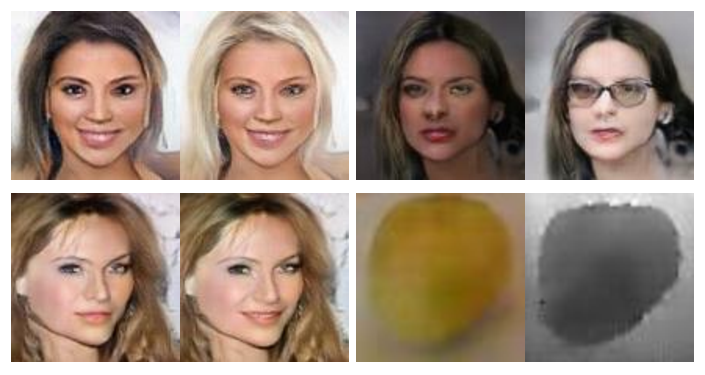
\includegraphics[trim=0.0in 0.0in 0.0in 0in, width=0.99\textwidth]{result_transfer_tight.pdf}    
\captionof{figure}{\small Cross-domain image transformation. For each pair, left is the input; right is the transformed image.}
\label{fig::result_transfer}
\end{minipage}
\end{table}